\chapter{Grundlagen der medizinischen Bildverarbeitung}
\addthumb{Grundlagen der medizinischen Bildverarbeitung}{\huge{\textbf{\thechapter.}}}{white}{haw_rot}

\section{Bildgewinnung und bildgebende Verfahren}

\section{DICOM}
Der Name DICOM steht für \textit{Digital Imaging and COmmunication in Medicine}. Der Umgang mit diesem Standard ist essentieller Bestandteil der zu entwickelnden Software. Pianykh\cite{pianykh:dicom} beschreibt im ersten Kapitel, dass DICOM nicht nur aus Pixel und deren zugehörigen Werten besteht. Wie der Name sagt, ist auch die Kommunikation fest im Standard verankert. Damit ist die Übertragung der Daten von medizinischen Geräten(Modalitäten) zum zentralen Speicher und deren Verteilung gemeint. Des weiteren spielt die dauerhafte Speicherung der digitalen Aufnahmen eine große Rolle. Daher wird im gleichen Zug mit DICOM immer ein PACS genannt. Die Abkürzung PACS bedeutet \textit{Picture Archiving and Communication System} und besteht sowohl aus Hardware (Server, Speicherung) als auch Software(Verteilung und Kommunikation).\\
Abbildung \ref{communication} illustriert das Zusammenspiel des DICOM-Standards und dem zentralen Datenspeicher. Zuerst wird mittels der Modalitäten(z.B. mit dem Computertomographen oder einem Ultraschallgerät) die digitale Aufnahme erzeugt. Danach wird das Bild vom Gerät an das PACS gesendet. Hier werden die Aufnahmen und Patientendetails in die Datenbank und den Speicher abgelegt. Wird eine Aufnahme benötigt können Clients Anfragen mit beispielsweise dem Patientennamen stellen und erhalten die zugehörige Serie mit der digitalen Aufnahme.

\begin{figure}[htbp]
  \vspace{0.5cm}
  \centering
  \fbox{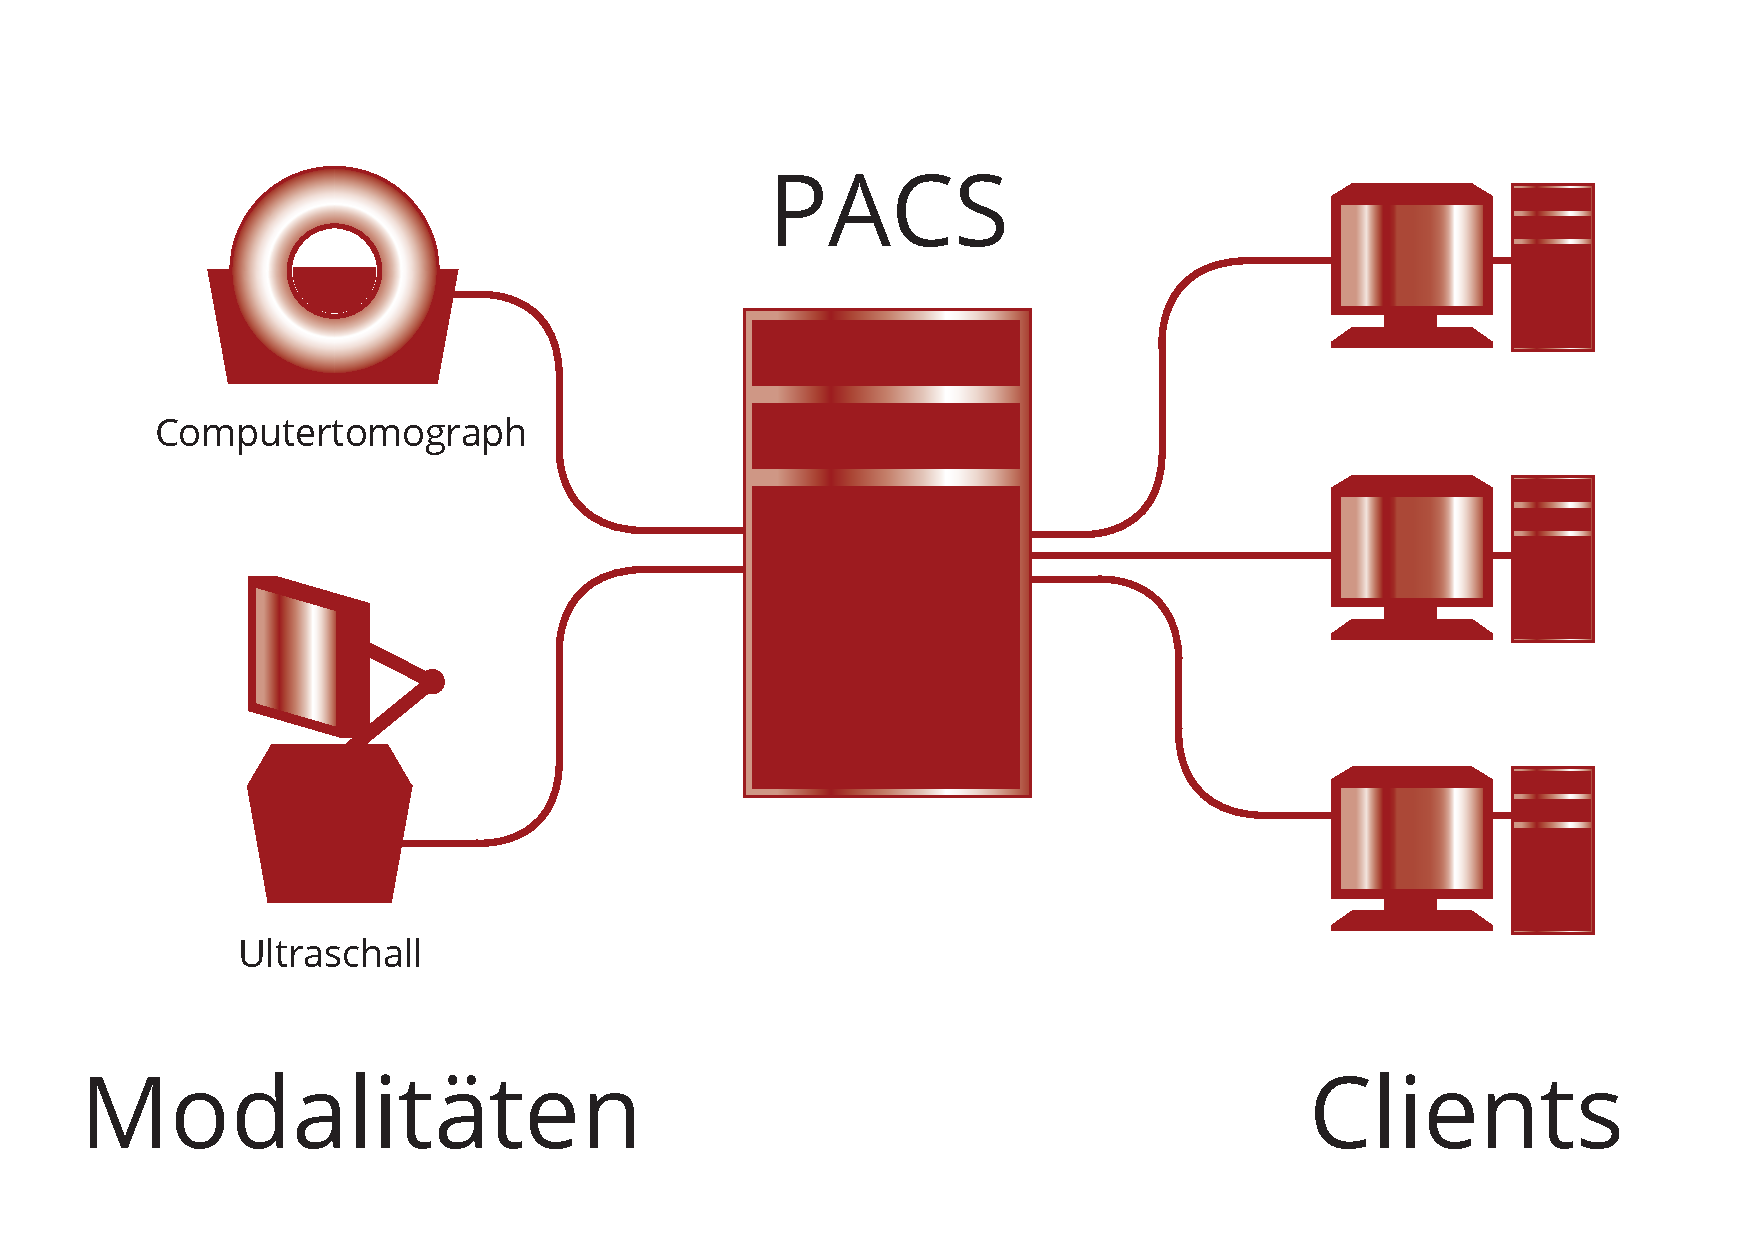
\includegraphics[angle=0,width=12cm]{./img/communication.pdf}}
  \caption{Kommunikationsprozess von Aufnahme zur Verarbeitung}
  \label{communication}
  \vspace{0.5cm}
\end{figure}

DICOM\footnote{Unter ftp://medical.nema.org/medical/dicom/ lässt sich der aktuelle Standard abrufen. Die Kapitel befinden sich im Ordner zum jeweiligen Jahr der Veröffentlichung. Aktuell sind die Dokumente von 2011.} ist daher nicht nur ein einzelner Standard, sondern verknüpft die standardisierte 
\begin{itemize}
\item Kommunikation,
\item Erzeugung der Bilddaten,
\item und Speicherung.
\end{itemize}
Im Rahmen dieser Abschlussarbeit liegt der Fokus auf den Bilddaten, daher wird auf die Kommunikation- und Speicheraspekte nicht im Detail eingegangen.

\subsection{Die Dicom Information Object Definitionen}
Bevor die Pixeldaten genauer betrachtet werden können, muss der prinzipielle Aufbau der Dicomobjekte beschrieben werden. Teil 3 des Standards\cite[A.1.2]{dicom:iod} zeigt den relationalen Aufbau der Dicomobjekte. Vereinfacht können die elementaren Informationsobjekte in drei Teile aufgeteilt werden.

\begin{itemize}
	\item \textbf{Patient}\\
	Der Patient steht in der Hierarchie an oberster Stelle und ist die Grundlage für eine oder mehrere Studien(Study).
	\item	\textbf{Study}\\
	Study symbolisiert eine medizinische Studie. Eine Studie ist eine Sammlung von mehreren Serien, die von Modalitäten wie CT und MR aufgezeichnet werden. Eine Studie ist exakt einem Patient zugeordnet.
	\item \textbf{Series}\\
	Eine Serie ist ein Folge von Bildern, die von einer Modalität erzeugt wird. Die Aufnahmen eines CT werden einer Serie zugeordnet. Jede Serie gehört zu nur einer Studie.
	\item \textbf{Image, Real World Values}\\
	Auf der unteren Hierarchiestufe stehen Objekte wie Bilddaten oder die Lage des Patienten im Raum während der Aufnahme. Ein Bild wird genau einer Serie zugeordnet.
\end{itemize}

Aus diesen vier elementaren Objekten ergibt sich folgende Informationsstruktur für Dicomobjekte, die in Abbildung \ref{ermodel} als Entity-Relationship-Modell\footnote{Ein ER-Modell beschreibt die Beziehungen der Elemente zueinander. Dieser Diagrammtyp wird unter Anderem häufig beim Entwickeln der Struktur einer relationalen Datenbank verwendet} verdeutlicht wird.

\begin{figure}[htbp]
  \vspace{0.5cm}
  \centering
  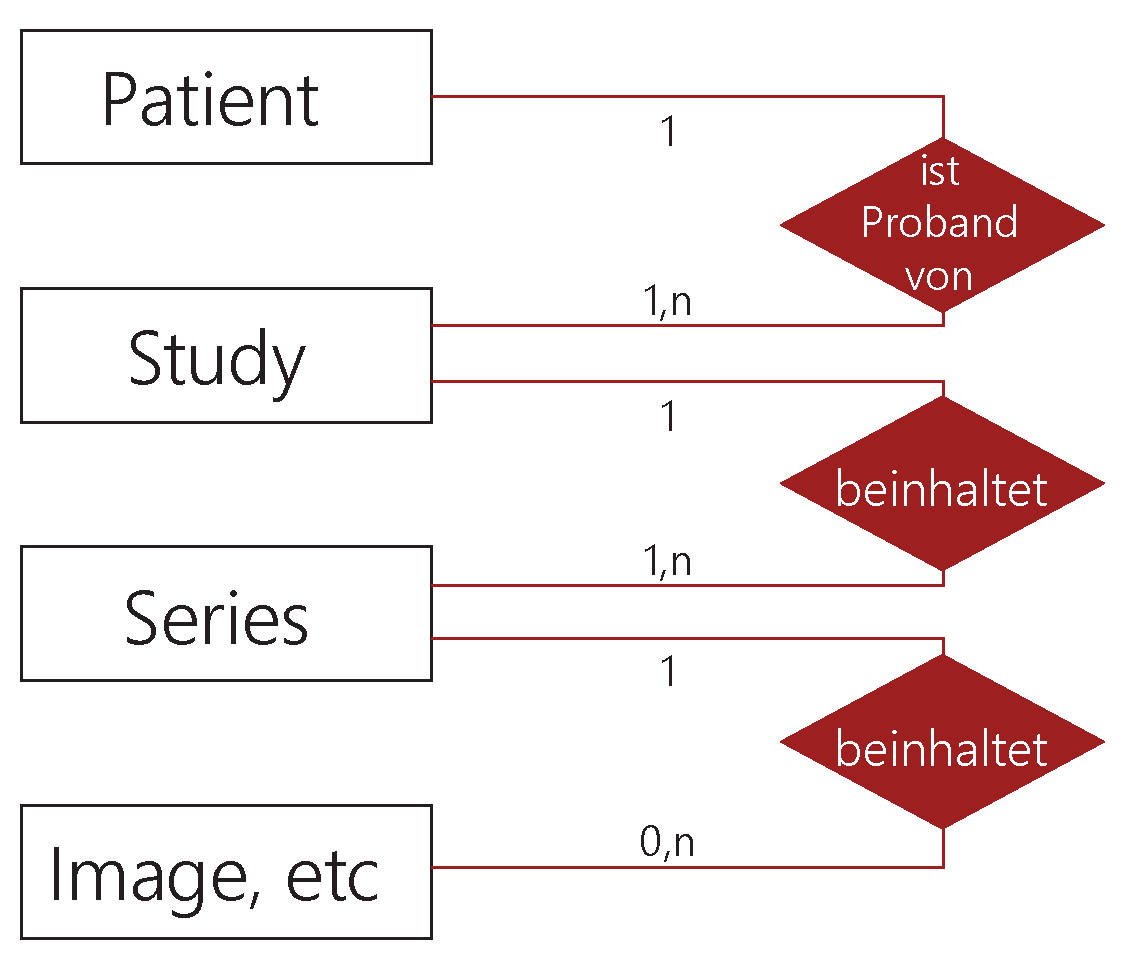
\includegraphics[angle=0,width=8cm]{./img/ermodel.pdf}
  \floatfoot{Vorlage für diese Darstellung ist die Grafik in \cite[A.1.2]{dicom:iod}}
  \caption{Vereinfachte Darstellung der Informationsobjekthierarchie von Dicomelementen}
  \label{ermodel}
  \vspace{0.5cm}
\end{figure}

Der DICOM-Viewer OsiriX bietet auf der Herstellerseite\footnote{http://www.osirix-viewer.com/datasets/} die Möglichkeit Testdaten zu beziehen. Betrachtet man die Repräsentation der Daten auf der Festplatte hält sich die Ordnerstruktur an obiges ER-Modell.\\
Abbildung \ref{filesystemrep} zeigt eine schmatische Darstellung der Dateien. Die Beispieldaten von OsiriX bestehen aus einem Patient names \glqq Brebix\grqq, dem eine Studie sowie zwei Serien à 100 Aufnahmen zugeordnet werden.

\tikzstyle{every node}=[draw=black,thick,anchor=west]
%\tikzstyle{selected}=[draw=red,fill=red!30]
\tikzstyle{optional}=[dashed,fill=gray!50]
\begin{figure}[htbp]
\centering
\caption{Repräsentation der Information Objekte im Dateisystem}
\label{filesystemrep}
\begin{tikzpicture}[%
  grow via three points={one child at (0.5,-0.7) and
  two children at (0.5,-0.7) and (0.5,-1.4)},
  edge from parent path={(\tikzparentnode.south) |- (\tikzchildnode.west)}]
  \node {Dicom Ordner}
    child [missing] {}
    child { node {BREBIX - Patient}
    	child [missing] {}
    	child { node{CT10 ponction foie - Studie}
    		child [missing] {}
    		child { node {DEF FOIE ART. - 107198 - Serie}
    			child{node[optional]{IM-0001-0001.dcm}}
    			child{node[optional]{...}}
    			child{node[optional]{IM-0001-0100.dcm}}
    		}
    		child [missing] {}				
    		child [missing] {}				
    		child [missing] {}
    		child [missing] {}
    		child { node {DEF. VEINEUX - 107205 - Serie}
    		    child{node[optional]{IM-0001-0001.dcm}}
    		    child{node[optional]{...}}
    		    child{node[optional]{IM-0001-0100.dcm}}
    		}
    		child [missing] {}
    	}
    };		
\end{tikzpicture}
\end{figure}

Bei näherem Hinsehen fällt auf, dass die Dateinamen beider Serien des Patienten identisch sind. Eine korrekte Zuordnung von DICOM-Dateien zur Serie ist daher nicht immer garantiert. Unabhängig von einer Repräsentation im Dateisystem oder Pfadangaben in der Datenbank eines PACS ist das Vertrauen auf Dateipfade unsicher, da über eine einfache Dateimanipulation die Zuordnung nicht mehr hergestellt werden kann.\\
Um eine zuverlässige Verknüpfung zu gewährleisten besitzt jeder Patient\footnote{Identifikationsnummern sind meist nur innerhalb einer Institution oder Krankenhauses einzigartig}, jede Studie und Serie eine Eindeutige Identifikationsnummer. Diese Art der Informationen wird in den atomaren Dateien mit Hilfe von Einträgen aus dem DICOM Data Dictionary\cite{dicom:dd} hinterlegt.
